\documentclass[11pt]{article}

\usepackage[left=1in, right=1in, top=1in, bottom=1in, paperwidth=8.5in, paperheight=69in]{geometry}

\usepackage{graphics,epsfig,graphicx,float,subfigure,color}
\usepackage{algorithm,algorithmic}
\usepackage{amsmath,amssymb,amsbsy,amsfonts,amsthm}
\usepackage[small,bf,up]{caption}

\usepackage{soul}
\usepackage{comment}
\usepackage{url}
\usepackage{boxedminipage}
\usepackage[sf,bf,small]{titlesec}
\usepackage[textsize=footnotesize]{todonotes}
\usepackage[plainpages=false, colorlinks=true,
   citecolor=blue, filecolor=blue, linkcolor=blue,
   urlcolor=blue]{hyperref}

\usepackage{amsmath}
\usepackage{xcolor} 

\newcommand{\bdm}{\begin{displaymath}}
\newcommand{\edm}{\end{displaymath}}

\newcommand{\ben}{\begin{enumerate}}
\newcommand{\een}{\end{enumerate}}

\newcommand{\p}{\partial}
\newcommand{\bs}{\boldsymbol}

\usepackage{amssymb}

\parskip 1ex

\parindent 0ex

\begin{document}
\pagestyle{empty}

\begin{center}
{\large {\bf MATH 140: Mathematical Methods for Optimization}}\\
{\bf Assignment 3---Spring 2024}\\
{\bf Due February 06, 2024} \\
{\textcolor{red}{\bf By:Ronald Nap}}
\end{center}

\begin{enumerate}

\item ({\bf 5 Points}) (Optional, extra credit) Prove that if $f(x)$
  is convex, then
  $$
  ( \nabla f(y) - \nabla f(x) )^T (y-x) \ge 0.
  $$
  In the one-dimensional case, represent this theorem pictorially.


\begin{enumerate}
    \item[\textcolor{red}{Solution:}] 
    \textcolor{red}{
    To prove that if $f(x)$ is convex, then
    \[
    ( \nabla f(y) - \nabla f(x) )^T (y-x) \ge 0,
    \]
    we start with the definition of convexity. A function $f: \mathbb{R}^n \to \mathbb{R}$ is convex if for any $x, y \in \mathbb{R}^n$ and $\lambda \in [0, 1]$, the following holds\footnote{Resource utilized for: \href{https://www.princeton.edu/~aaa/Public/Teaching/ORF523/S16/ORF523_S16_Lec7_gh.pdf}{Problem \#1}.}:
    \[
    f(\lambda x + (1-\lambda)y) \le \lambda f(x) + (1-\lambda)f(y).
    \]
    Using the gradient, we express a property of convex functions:
    \[
    f(y) \ge f(x) + \nabla f(x)^T(y-x).
    \]
    Consider $g(t) = f(x + t(y-x))$ for $t \in [0,1]$. Since $f$ is convex, so is $g(t)$, and thus:
    \[
    g'(t) = \nabla f(x + t(y-x))^T (y-x)
    \]
    is non-decreasing. This implies $g'(1) \ge g'(0)$, or:
    \[
    \nabla f(y)^T (y-x) \ge \nabla f(x)^T (y-x),
    \]
    leading to:
    \[
    (\nabla f(y) - \nabla f(x))^T (y-x) \ge 0,
    \]
    }

    \begin{figure}[H]
    \centering
    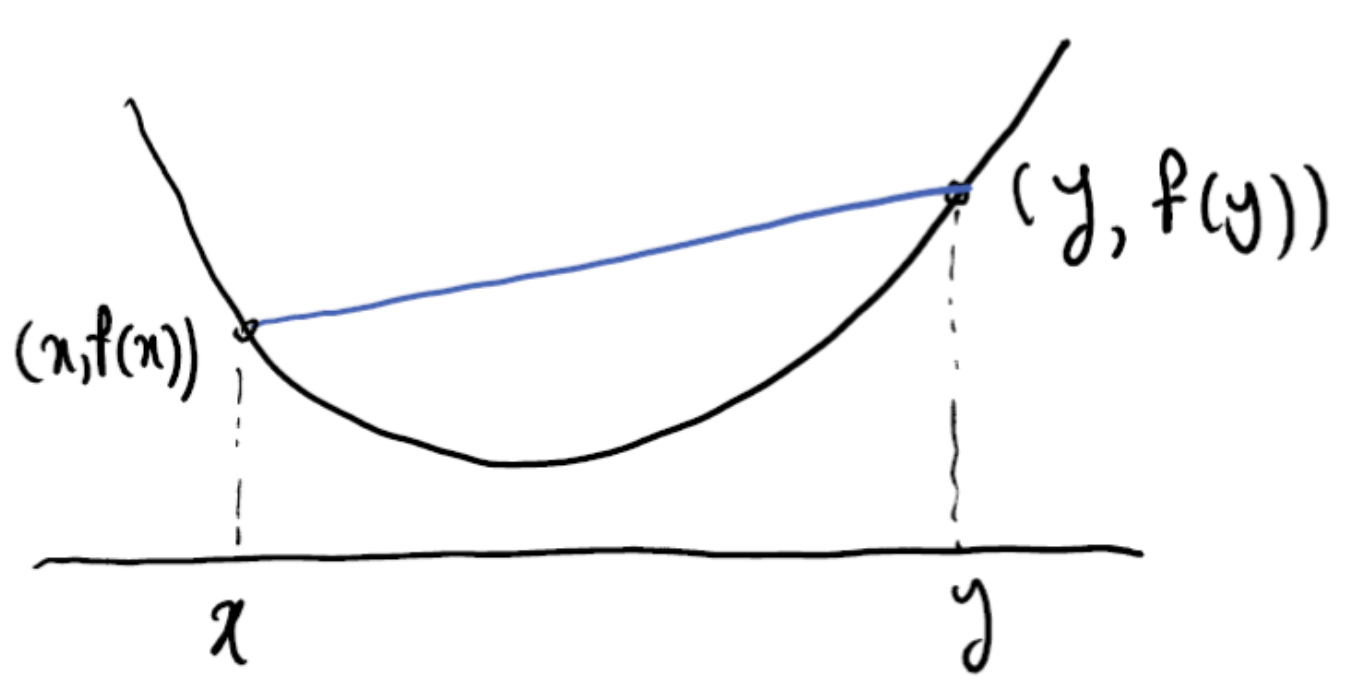
\includegraphics[width=\textwidth]{1.png} 
    \end{figure}

\end{enumerate}



\item {\bf (5 Points)} Due to the finite precision in floating point
  number representation, there are gaps between consecutive
  numbers. The size of these gaps depends on the size of the number
  and on the precision (e.g., double or single precision). MATLAB
  provides the function \texttt{eps($\cdot$)} (the analogue in NumPy
  is the function \texttt{spacing}), which returns, for a number, the
  distance to the next floating point number in the same precision.
  Using the form of double and single floating point number
  representation, explain the values you find for\\[1ex] \texttt{
    eps(1),\footnote{This value, \texttt{eps(1)} = \texttt{eps}
      $\approx 2.22\times 10^{-16}$ is usually referred to as machine
      epsilon, and it gives an indication of the rounding error when
      dealing with double precision floating point
      numbers.}\\ eps(single(1)),\footnote{Note that the MATLAB
      command \texttt{single} switches to single
      precision.}\\ eps($2^{40}$),\\ eps(single($2^{40}$)).}

    \begin{enumerate}
        \item[\textcolor{red}{Solution:}] \textcolor{red}{This output demonstrates the concept of machine epsilon and the differences in precision between single and double precision floating point representations. For the number 1.0, the double precision epsilon is approximately 2.22e-16, indicating a higher precision, while the single precision epsilon is approximately 1.19e-07, indicating a lower precision. Similarly, for the number $2^{40}$, we see a larger gap in the representable numbers, with the double precision having a gap of about 0.000244 and the single precision having a much larger gap of 131072.0}
    \end{enumerate}

    \begin{figure}[h]
    \centering
    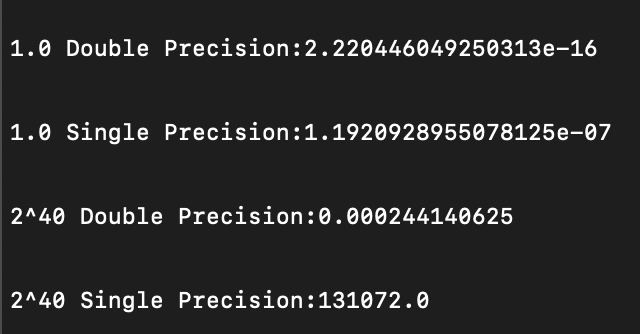
\includegraphics[width=\textwidth]{2.png} 
    \end{figure}


  \item {\bf (5 Points)} Consider $f(x) = \tan x$, and point $a =
  \frac{\pi}{4}$ in the interval $[\alpha, \beta] = [0,
    \frac{\pi}{4}]$.
    
  \begin{enumerate}
  \item Compute the Taylor polynomials $p_n(x)$, $n = 1, 2$ about
    a point $a$.
    \begin{enumerate}
        \item[\textcolor{red}{Solution:}] \textcolor{red}{The first Taylor polynomial $p_1(x)$ is $f(a) + f'(a)(x-a)$, where $f'(x) = \sec^2 x$. At $a$, $f'(a) = 2$. Thus, $p_1(x) = 1 + 2(x - \frac{\pi}{4})$. The second Taylor polynomial $p_2(x)$ includes the second derivative $f''(x) = 2\sec^2 x \tan x$, so $f''(a) = 4$. Therefore, $p_2(x) = 1 + 2(x - \frac{\pi}{4}) + 2(x - \frac{\pi}{4})^2$.}
    \end{enumerate}

  \item Plot the function $f(x)$ and the Taylor polynomial $p_n(x)$,
    $n = 1, 2$ over the interval $[\alpha, \beta]$ (in the same
    plot).

    \begin{figure}[h]
    \centering
    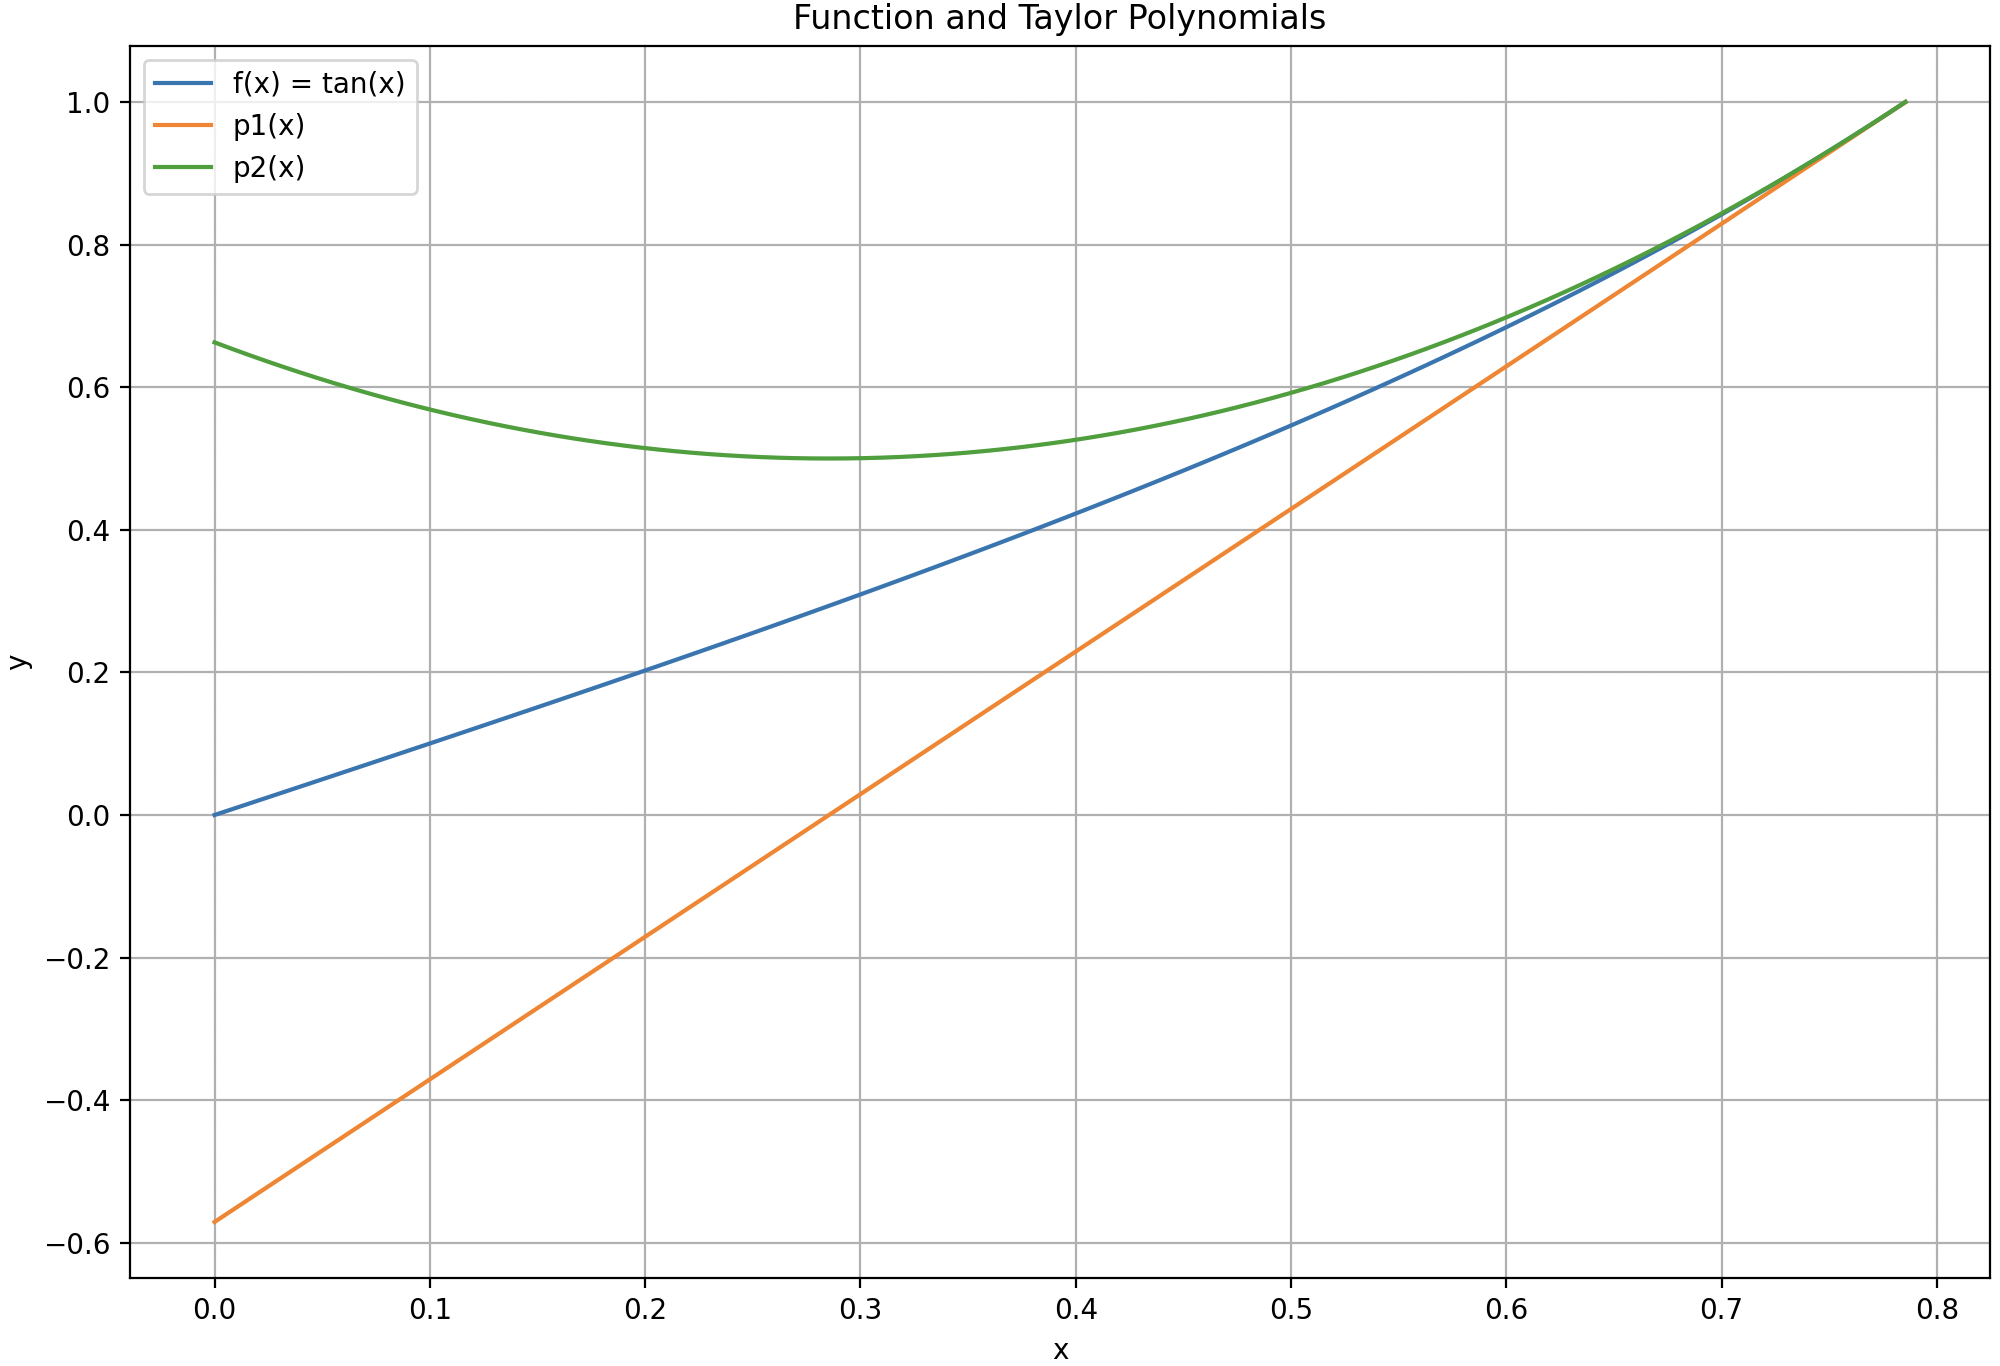
\includegraphics[width=\textwidth]{3b.png} 
    \end{figure}

  \item Plot the reminders $r_n(x) = f(x) - p_n(x)$, $n = 1, 2$
    over the interval $[\alpha, \beta]$ (in the same plot).

    \begin{figure}[h]
    \centering
    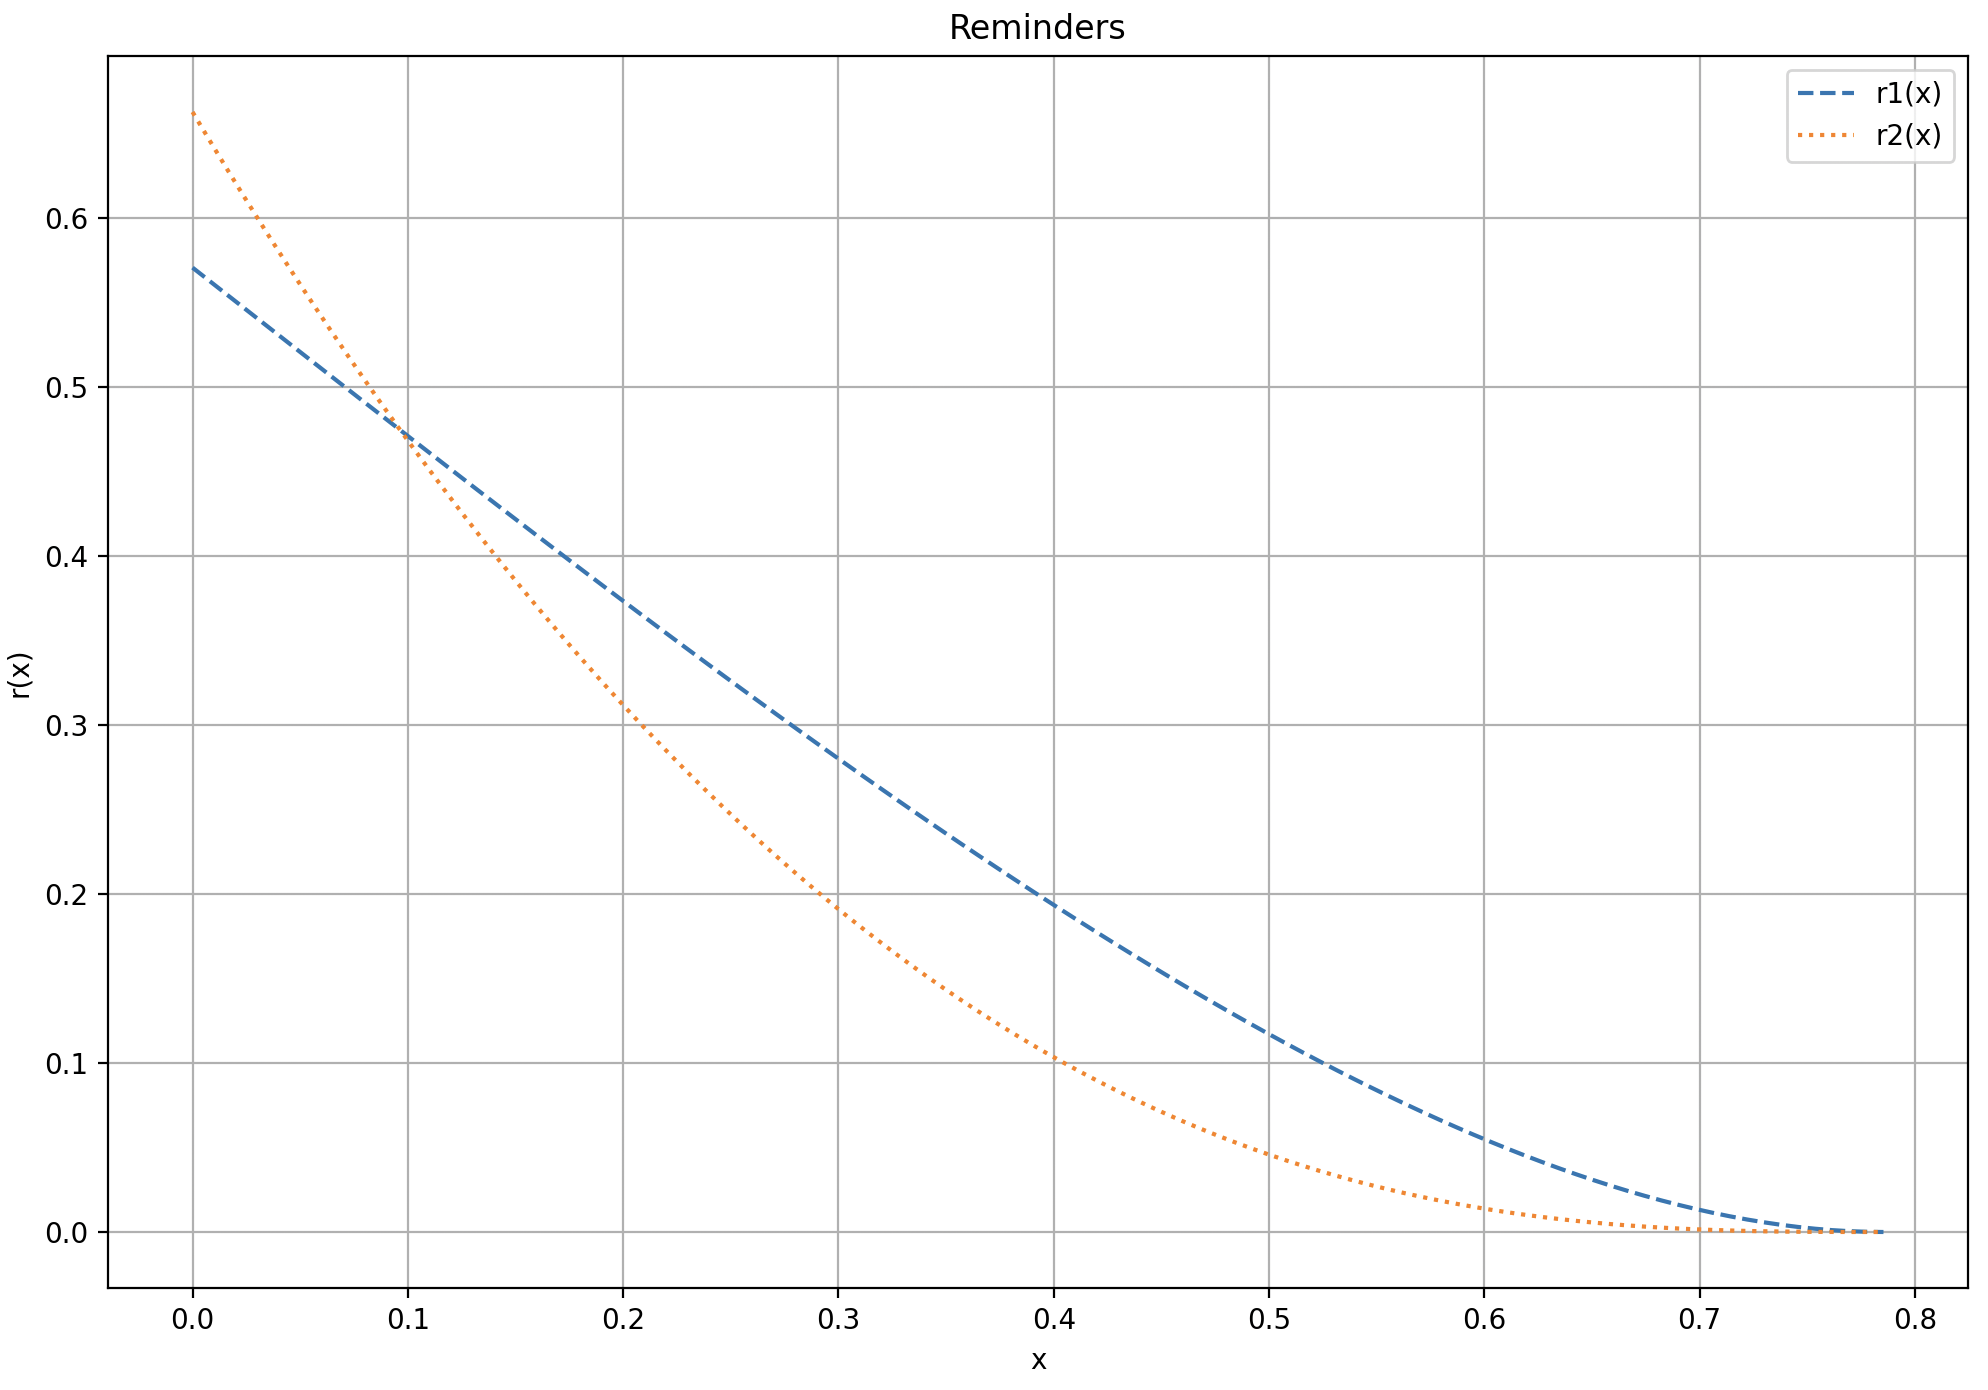
\includegraphics[width=\textwidth]{3c.png} 
    \end{figure}
    
  \item Bound the absolute value of the reminders $r_n(x) = f(x) -
    p_n(x)$, $n = 1, 2$. Are the reminders obtained in (c) less
    than your theoretica bounds for all $x$ in $[\alpha, \beta]$?

\begin{enumerate}
    \item[\textcolor{red}{Solution:}] 
    \textcolor{red}{
    To bound the absolute value of the remainders $r_n(x) = f(x) - p_n(x)$ for $n = 1, 2$, we use Taylor's theorem with the Lagrange form of the remainder. For $p_1(x)$, the bound is:
    \[
    |r_1(x)| \leq \frac{|f''(\xi_1)|}{2!} (x - a)^2,
    \]
    where $\xi_1 \in [\alpha, \beta]$ and $|f''(\xi_1)|$ is the maximum value of the second derivative on the interval, which was computed to be 2 (Figure a). For $p_2(x)$, the bound is:
    \[
    |r_2(x)| \leq \frac{|f'''(\xi_2)|}{3!} (x - a)^3,
    \]
    where $\xi_2 \in [\alpha, \beta]$ and $|f'''(\xi_2)|$ is the maximum value of the third derivative on the interval, which was computed to be 12.83 (Figure b). Therefore, the actual bounds for the remainders are:
    \[
    |r_1(x)| \leq \frac{2}{2} (x - \frac{\pi}{4})^2,
    \]
    \[
    |r_2(x)| \leq \frac{12.83}{6} (x - \frac{\pi}{4})^3.
    \]
    }
    \begin{figure}[H]
    \centering
    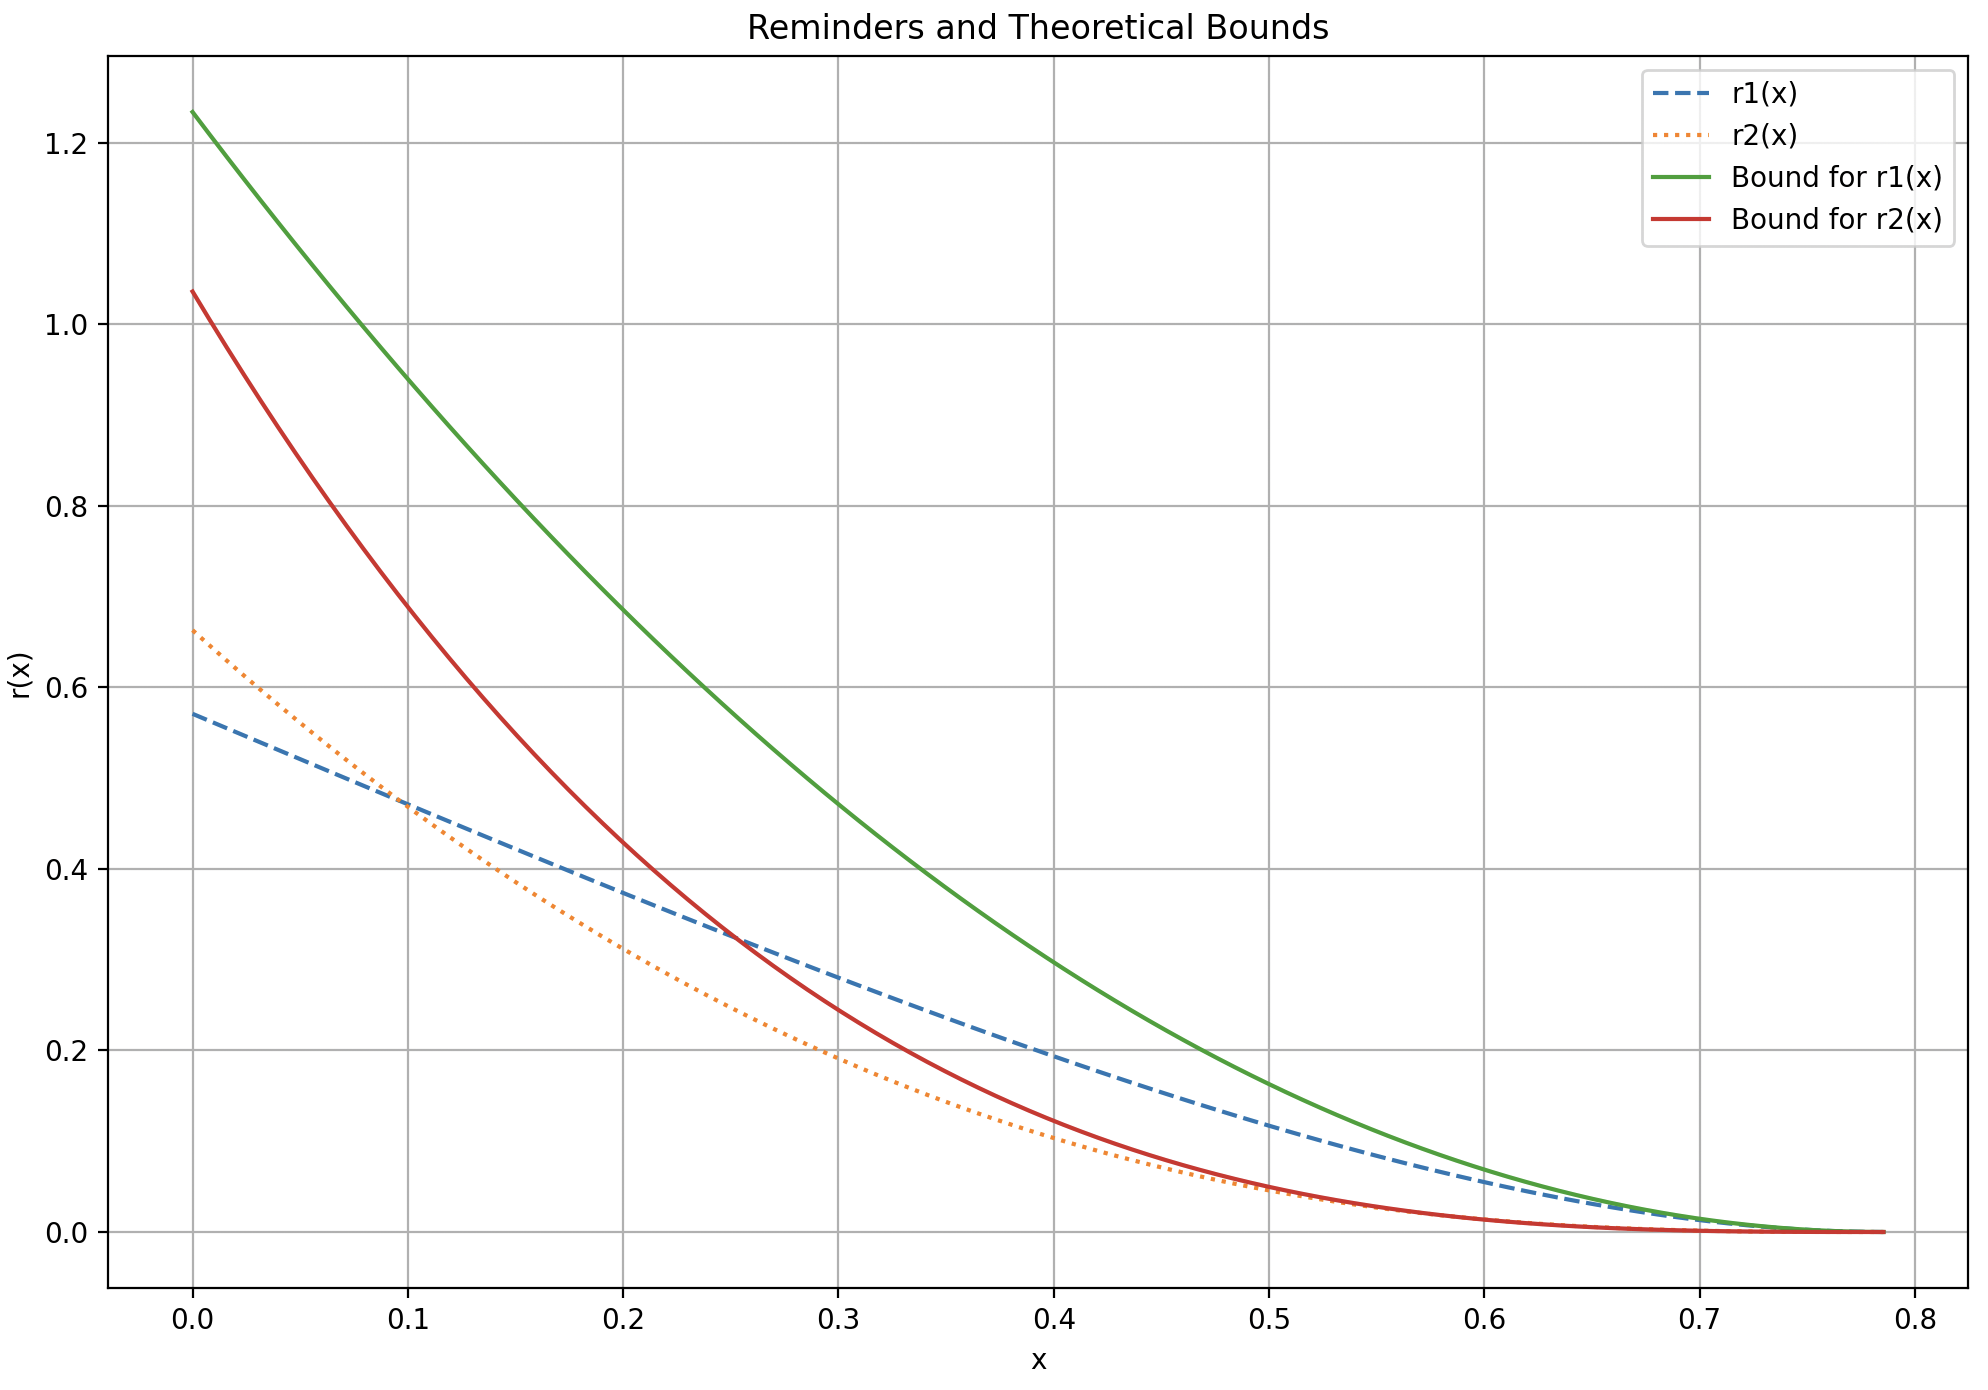
\includegraphics[width=\textwidth]{3d.png} 
    \centering
    \begin{tabular}{cc}
    \\[.2cm]
    \hspace{-.25cm} 
    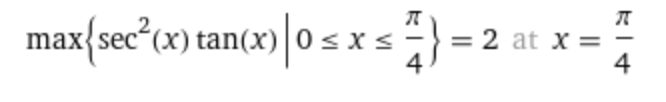
\includegraphics[width=7.45cm]{max1.png} \hspace{-.5cm} &  
    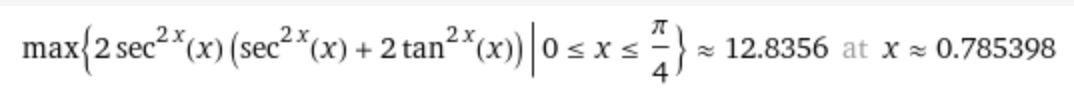
\includegraphics[width=9.45cm]{max2.png}  \\       
    (a) \href{https://www.wolframalpha.com/input?i2d=true&i=find+maximum+of+Power%5Bsec%5C%2840%29x%5C%2841%29%2C2%5D%5C%2840%29tan%5C%2840%29x%5C%2841%29%5C%2841%29+on+%5C%2891%290%5C%2844%29Divide%5Bpi%2C4%5D%5C%2893%29%5C%2844%29}{For $|f''(\xi_1)|$} &  (b) \href{https://www.wolframalpha.com/input?i2d=true&i=find+maximum+of+2+Power%5Bsec%2C2%5C%2840%29x%5C%2841%29%5D+%5C%2840%29Power%5Bsec%2C2%5C%2840%29x%5C%2841%29%5D+%2B+2+Power%5Btan%2C2%5C%2840%29x%5C%2841%29%5D%5C%2841%29+on+%5C%2891%290%5C%2844%29Divide%5Bpi%2C4%5D%5C%2893%29%5C%2844%29}{For $|f'''(\xi_2)|$}  \\
    \end{tabular}
    \end{figure}    
\end{enumerate}



    
  \end{enumerate}



 \item {\bf (5 Points)} Consider the problem of approximating the
   derivative $f'(x_0)$ of a given smooth function $f(x)$ at the point
   $x=x_0$. For intance let $f(x) = \sin(x)$ be defined on the real
   line $-\infty < x < \infty$, and set $x_0 = 1.2$ thus $f(x_0 =
   \sin(1.2) \approx 0.932\dots$. Follow the example in the discussion
   session, where we used Taylor's series for the approximation, and
   adapt the a matlab code shared in catcourses to reproduces the
   loglog plot and the error table we discussed in the discussion
   session. That is, compute the absolute error for a sequence of
   decreasing $h$ values and write these into a table. Also, plot on a
   loglog plot the absolute error versus $h$. Discuss your results.


    \begin{figure}[H]
    \centering
    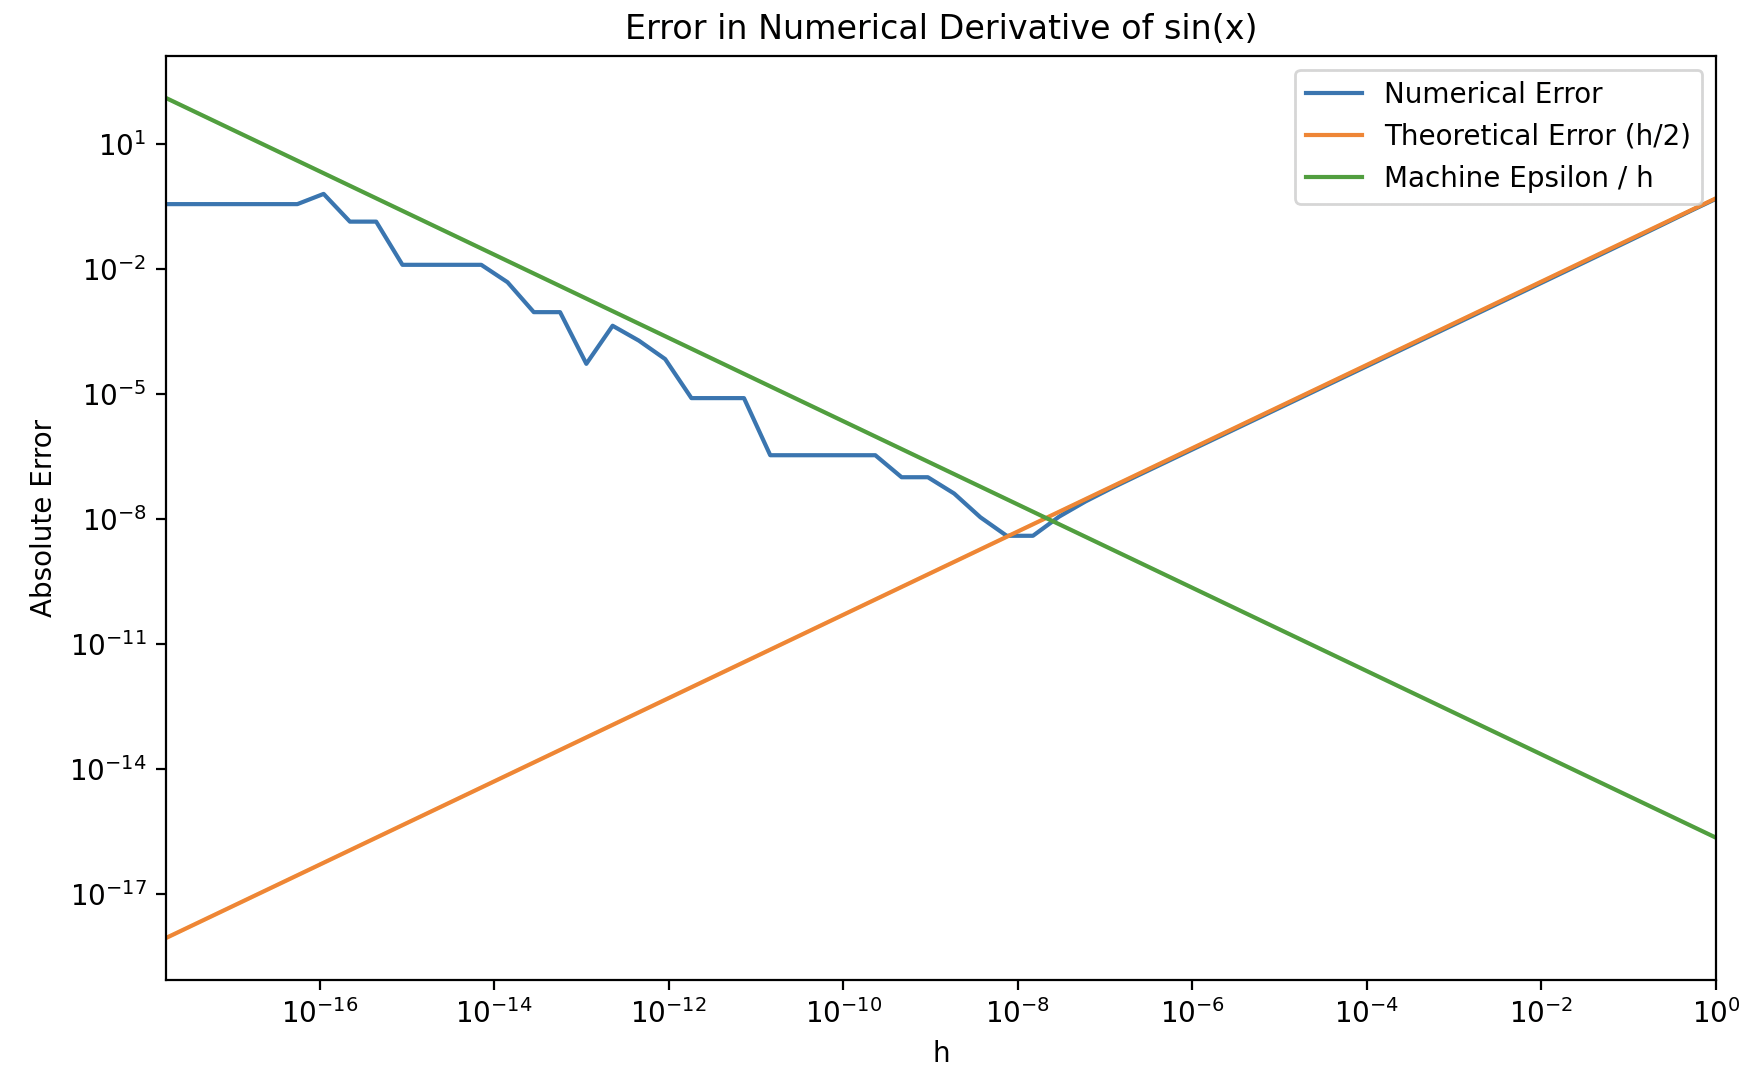
\includegraphics[width=\textwidth]{4.png} 
    \end{figure}


\begin{enumerate}
    \item[\textcolor{red}{Summary:}] 
    \textcolor{red}{
      The log-log plot showcases the relationship between step size \( h \) and the absolute error in numerical derivative approximation of \( \sin(x) \) at \( x = 1.2 \). As \( h \) decreases, the numerical error diminishes until it reaches a minimum threshold, beyond which the error starts to rise due to the limitations of machine precision. The plot reveals the nature of errors in numerical differentiation, the approximation error, which lessens with finer step size, and the round-off error, which escalates when \( h \) is too small. This graph underscores the importance of balancing step size to minimize the total error, exemplifying the compromise between approximation accuracy and computational limitations of floating-point arithmetic. It illustrates the optimum \( h \) region where the derivative estimation is most precise before the effects of finite precision become predominant.}
\end{enumerate}

    \begin{figure}[H]
    \centering
    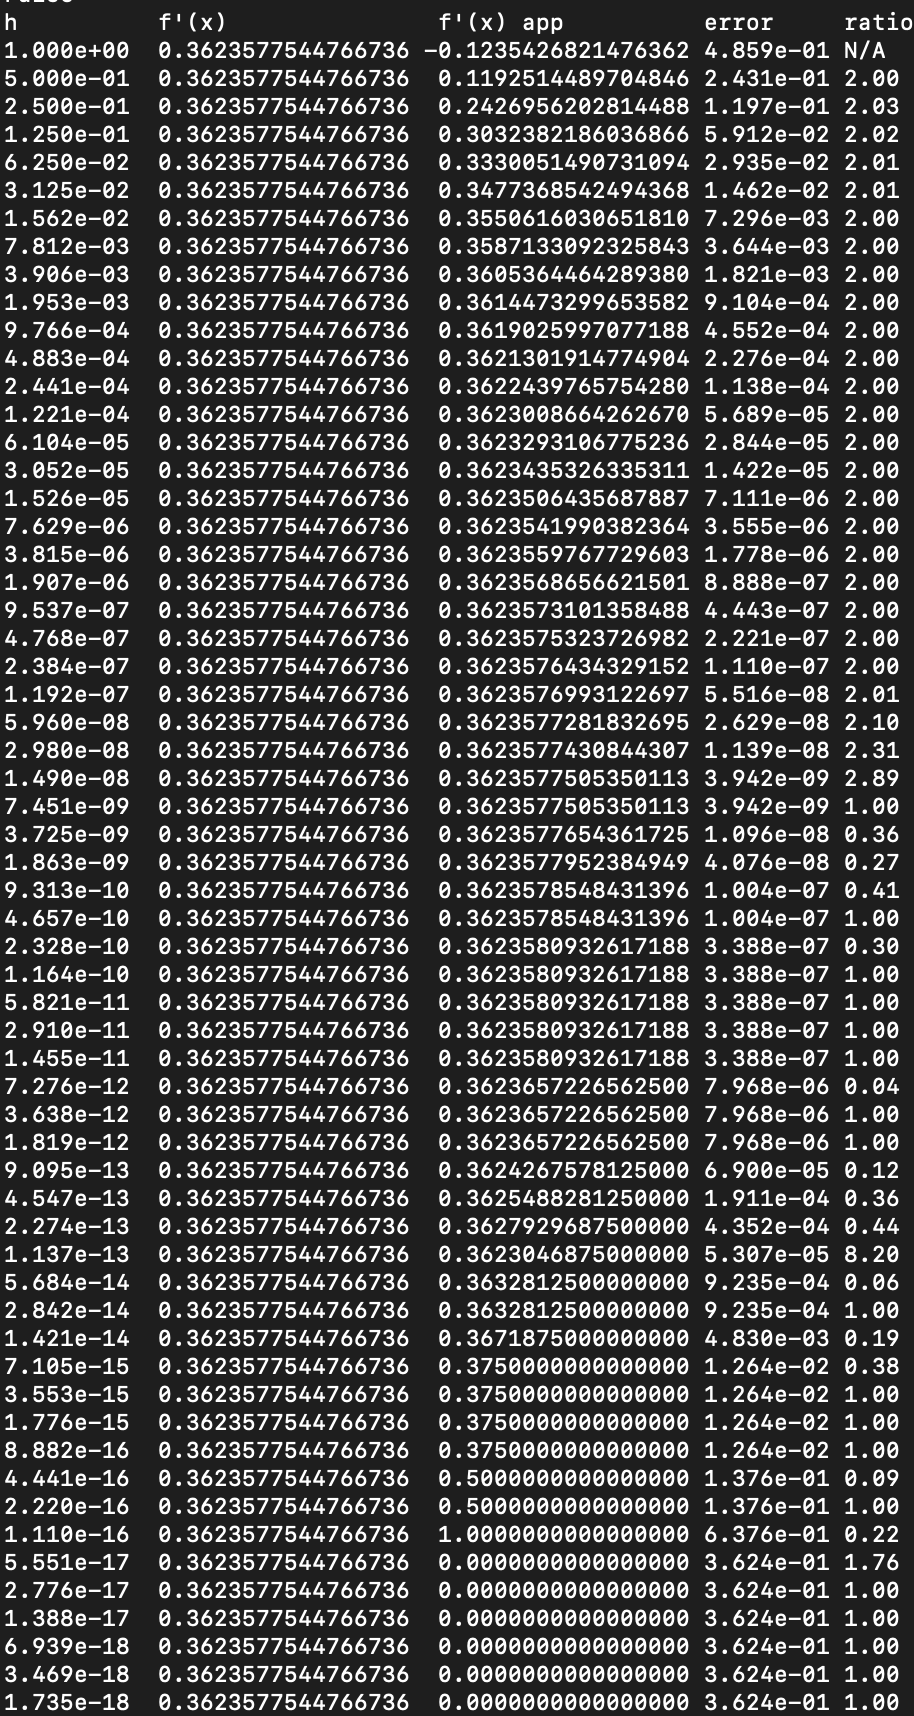
\includegraphics[width=\textwidth]{4b.png} 
    \end{figure}


  \item {\bf (5 Points)}
\begin{enumerate}
\item Read Section 2.3 in the NewtonsMethod-BurdenFaires file
  attached. Summarize and report on questions if you have any,
  otherwise no need to write up a summary, unless you'd like to.
\begin{enumerate}
    \item[\textcolor{red}{Summary:}] 
    \textcolor{red}{
  The Newton's Method section in the Burden and Faires document describes iterative techniques for finding function roots. Newton's Method uses tangents for fast convergence, requiring derivative calculations. The Secant Method omits derivatives, using secant lines instead, benefiting situations where derivatives are complex. It converges slower than Newton's but can be more practical. The Method of False Position also avoids derivatives and keeps the root within bounds, potentially increasing the number of steps needed.}
\end{enumerate}



\item Implement the Newton and Secant methods and test your code by
  applying it to solve Example 3 on page 74 in the
  NewtonsMethod-BurdenFaires file attached. If your code works
  properly, you should be able to reproduce columns three and four of
  Table 2.6 for both methods.

    \begin{figure}[H]
    \centering
    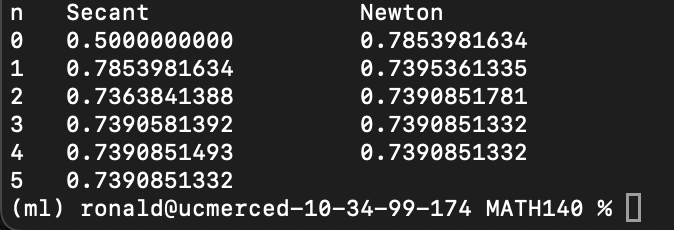
\includegraphics[width=\textwidth]{5b.png} 
    \end{figure}



\item Given your results above explain what advantages does Newton
  method have over Secant method and what advantages Secant method has
  over Newton's method.



\begin{enumerate}
    \item[\textcolor{red}{Pros and Cons:}] 
    \textcolor{red}{Newton's method offers rapid convergence with a precise initial guess and a differentiable function, making it highly efficient for well-behaved functions. However, its necessity for derivative calculation adds computational complexity and can be a significant limitation for complex functions. The Secant method, not requiring derivatives, is simpler and more versatile, especially for complicated functions. However, it generally converges slower than Newton's method and might fail with poorly chosen initial guesses.}
\end{enumerate}



  
\end{enumerate}
\end{enumerate}
\end{document}